\section{Medidas de dispersión}

\paragraph{Dispersión o variación}
Si bien las medidas de tendencia central nos dicen alrededor de que valores se concentra un arreglo de datos, las \emph{medidas de dispersión} nos dan una idea de que tan alejados están entre sí.





A continuación, veremos algunas medidas de dispersión comúnmente usadas en estadística.

\paragraph{Rango}
El \emph{rango}
de un conjunto de datos es la diferencia entre el mayor y el menor del conjunto.



\begin{ejemplo}
	El rango del conjunto 2,3,3,5,5,5,8,10,12 es $12-2=10.$
\end{ejemplo}


\paragraph{Desviación media}
La \emph{desviación media} o \emph{desviación promedio} de un conjunto de $N$ números $X_{1},...,X_{N}$ está definida como
\begin{align}
	DM=\dfrac{\sum \abs{X_{j}-\bar{X}}}{N}
\end{align}
donde $\bar{X}$ es la media aritmética de los números y $\abs{\cdot}$ denota el valor absoluto.


\begin{ejemplo}
	Encuentre la desviación media de la lista $2,3,6,8,11.$
\end{ejemplo}


\paragraph{Desviación estándar}
La \emph{desviación estándar} de un conjunto de $N$ números $X_{1},...,X_{N}$ se denota como $s$ y está definida por
\begin{align}
	s=\sqrt{\dfrac{\sum\left( X_{j}-\bar{X} \right)^{2}}{N}}=\sqrt{\sum\dfrac{x_{j}^{2}}{N}}
\end{align} donde $x_{j}:=X_{j}-\bar{X}.$


Si $X_{1},...,X_{N}$ se presentan con frecuencias $f_{1},...,f_{N}$ respectivamente, la desviación estándar se puede expresar como
\begin{align}
	s=\sqrt{\dfrac{\sum f_{j}\left( X_{j}-\bar{X} \right)^{2}}{N}}=\sqrt{\dfrac{\sum f_{j}x_{j}^{2}}{N}}
\end{align}


\begin{observacion}
	En ocasiones, $N$ se reemplaza por $N-1$ en las fórmulas anteriores, debido a que está definición aproxima mejor a la población de la que se ha obtenido la muestra. Pero para muestras muy grandes $N>30$ prácticamente no hay diferencia.
\end{observacion}


\paragraph{Varianza}
La \emph{varianza} de un conjunto de números se define como el cuadrado $s^{2}$ de la desviación estándar $s$.


\begin{observacion}
	En estadística, es importante distinguir entre la desviación estándar de una \emph{población} y una \emph{muestra}. Para distinguirla, en el primer caso utilizaremos $\s$ y en el segundo, continuaremos usando $s.$
\end{observacion}


\paragraph{Método abreviado}
\begin{align}
	s^{2}&=\overline{X^{2}}-\overline{X}^{2} \\
	&= E(X^2)-\left( E(X) \right)^{2}
	%\\ 
	%s^{2}&=\overline{d^{2}}-\overline{d}^{2}
\end{align}



En las distribuciones normales se tiene que
\begin{enumerate}
	\item $68.27\%$ de los datos está comprendido entre $\bar{X}\pm s.$
	\item $95.45\%$ de los datos está comprendido entre $\bar{X}\pm 2s.$
	\item $99.73\%$ de los datos está comprendido entre $\bar{X}\pm 3s.$
	
\end{enumerate}



Si $2$ conjuntos de $N_{1}$ y $N_{2}$ datos respectivamente tienen correspondientes $s_{1}^{2}$ y $s_{2}^{2}$ varianzas pero una misma media aritmética $\bar{X},$ entonces la varianza de la unión de ambos conjuntos es
\begin{align}
	s^{2}=\dfrac{N_{1}s_{1}^{2}+N_{2}s_{2}^{2}}{N_{1}+N_{2}}.
\end{align}

\paragraph{Teorema de Chebyshev}
Para $k>1,$ por lo menos $1-\dfrac{1}{k^{2}}$ de la distribución de problemaabilidad de cualquier variable aleatoria está a nomas  de $k$ desviaciones estándar de la media.

\subsection{Python}
[]{\texttt{numpy.std}}
\begin{lstlisting}[language=Python]
	numpy.std(a, axis=None, dtype=None, out=None, ddof=0,
	keepdims=<class numpy._globals._NoValue>)
\end{lstlisting}

Calcule la desviación estándar a lo largo del eje especificado.

Devuelve la desviación estándar, una medida de la propagación de una distribución, de los elementos de la matriz. La desviación estándar se calcula para la matriz aplanada de forma predeterminada, de lo contrario sobre el eje especificado.\footnote{https://docs.scipy.org/doc/numpy/reference/generated/numpy.std.html}

[]
\begin{lstlisting}[language=Python]
	import numpy as np
	
	a = np.array([[1, 2], [3, 4]])
	print np.std(a)
	#1.1180339887498949
	print np.std(a, axis=0)
	#array([ 1.,  1.])
	print np.std(a, axis=1)
	#array([ 0.5,  0.5])
\end{lstlisting}


[]
\begin{lstlisting}[language=Python]
	#In single precision, std() can be inaccurate:
	a = np.zeros((2, 512*512), dtype=np.float32)
	a[0, :] = 1.0
	a[1, :] = 0.1
	print np.std(a)
	#0.45000005
	
	#Computing the standard deviation in float64
	#is more accurate:
	print np.std(a, dtype=np.float64)
	#0.44999999925494177
\end{lstlisting}





\begin{problema}
	\label{problema:4.3}
	Encontrar el rango y las desviaciones media y estándar de los arreglos 
	\begin{enumerate}
		\item $12,6,7,3,15,10,18,5$ 
		\item $9,3,8,8,9,8,9,18.$
	\end{enumerate}
	
	Compruebe sus resultados con \texttt{Python.}
\end{problema}




\begin{problema}
	\label{problema:4.4}
	Encontrar las desviaciones media y estándar de las estaturas de 100 estudiantes de la siguiente tabla:
	\begin{figure}[ht]
		\centering
		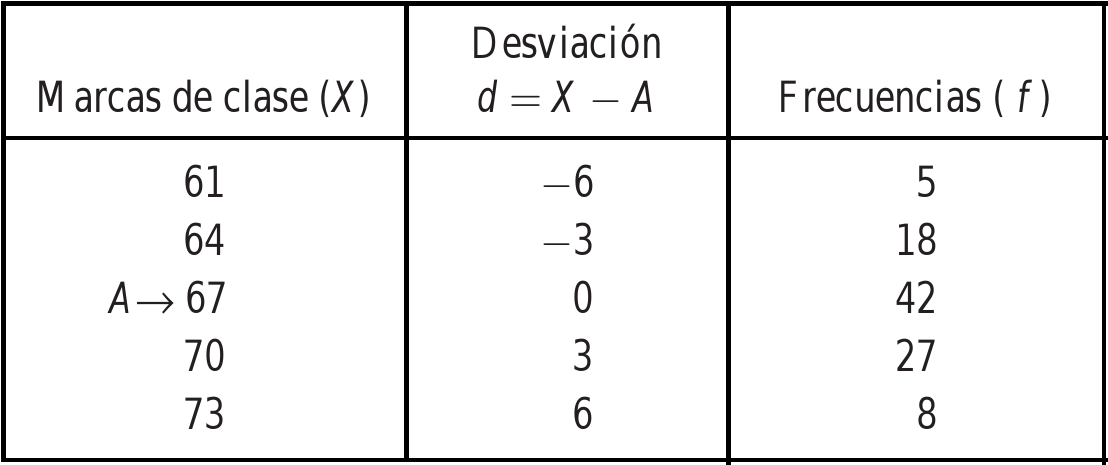
\includegraphics[width=10cm,keepaspectratio=true]{./images/tab0302.png}
		% tab0302.png: 0x0 pixel, 300dpi, 0.00x0.00 cm, bb=
		\label{tab:0302}
	\end{figure}
	
\end{problema}




\begin{problema}
	\label{problema:4.11}
	Encontrar las desviaciones media y estándar de las estaturas de 100 estudiantes de la siguiente tabla:
	\begin{figure}[ht]
		\centering
		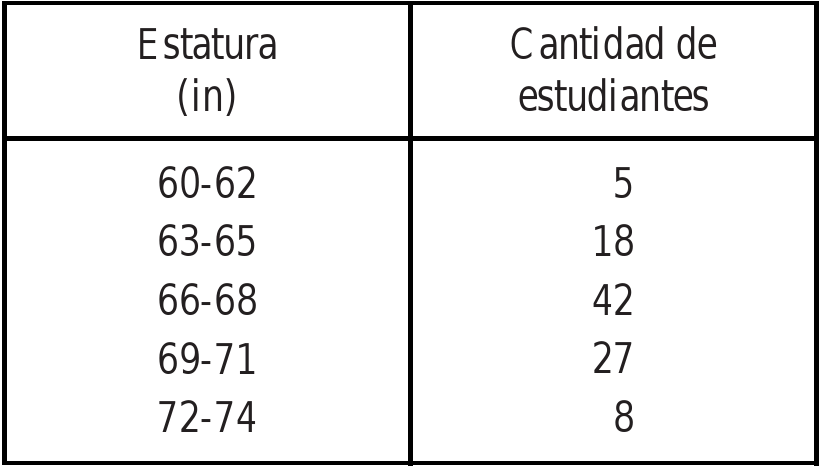
\includegraphics[height=5cm,keepaspectratio=true]{./images/tab0201.png}
		% tab0302.png: 0x0 pixel, 300dpi, 0.00x0.00 cm, bb=
		\label{tab:0201}
	\end{figure}
	
\end{problema}




\begin{problema}
	\label{problema:4.12}
	Demostrar que
	\begin{align}
		s &= \sqrt{\dfrac{\sum X^{2}}{N}-\left( \dfrac{\sum X}{N} \right)^{2}}&=
		\sqrt{\overline{X^{2}}-\overline{X}^{2}}\\
		s &= \sqrt{\dfrac{\sum fX^{2}}{N}-\left( \dfrac{\sum fX}{N} \right)^{2}}&=
		\sqrt{\overline{X^{2}}-\overline{X}^{2}}
	\end{align}
\end{problema}




\begin{problema}
	\label{problema:4.14}
	Utilizando las fórmulas anteriores, encuentre la desviación estándar de los datos en la tabla \ref{tab:0201}:
	\begin{figure}[ht]
		\centering
		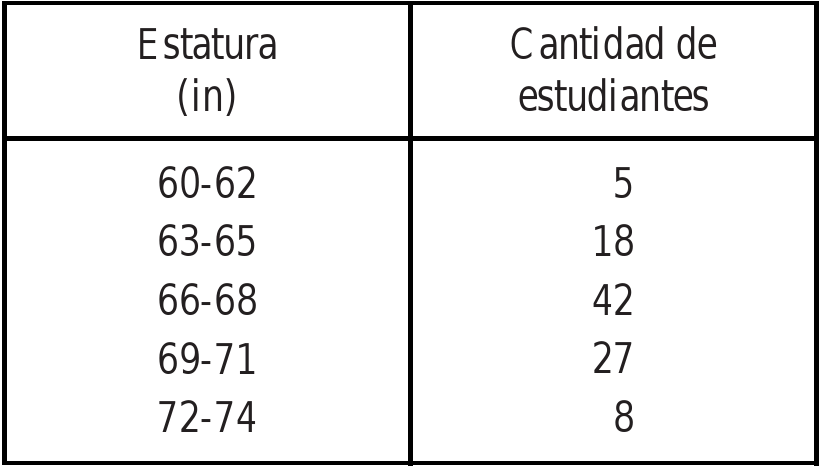
\includegraphics[height=5cm,keepaspectratio=true]{./images/tab0201.png}
		% tab0302.png: 0x0 pixel, 300dpi, 0.00x0.00 cm, bb=
		%\label{tab:0201}
	\end{figure}
	
\end{problema}




\begin{problema}
	\label{problema:4.15}
	Si $d=X-P$ son desviaciones de $X$ respecto a un pivote $P,$ demostrar que
	\begin{align}
		s=\sqrt{\dfrac{\sum fd^{2}}{N}-\left( \dfrac{\sum fd}{N} \right)^{2}}.
	\end{align}
\end{problema}



\begin{problema}
	\label{problema:4.17}
	Utilizando las fórmulas anteriores, encuentre la desviación estándar de los datos en la tabla \ref{tab:0201}:
	\begin{figure}[ht]
		\centering
		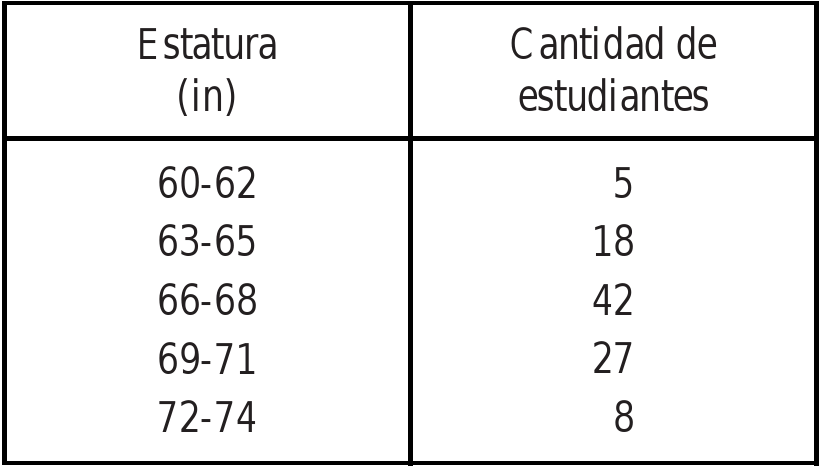
\includegraphics[height=5cm,keepaspectratio=true]{./images/tab0201.png}
		% tab0302.png: 0x0 pixel, 300dpi, 0.00x0.00 cm, bb=
		%\label{tab:0201}
	\end{figure}
	
\end{problema}




\begin{problema}
	\label{problema:4.18}
	Encuentre la media aritmética y  la desviación estándar de los siguientes datos:
	\begin{figure}[ht]
		\centering
		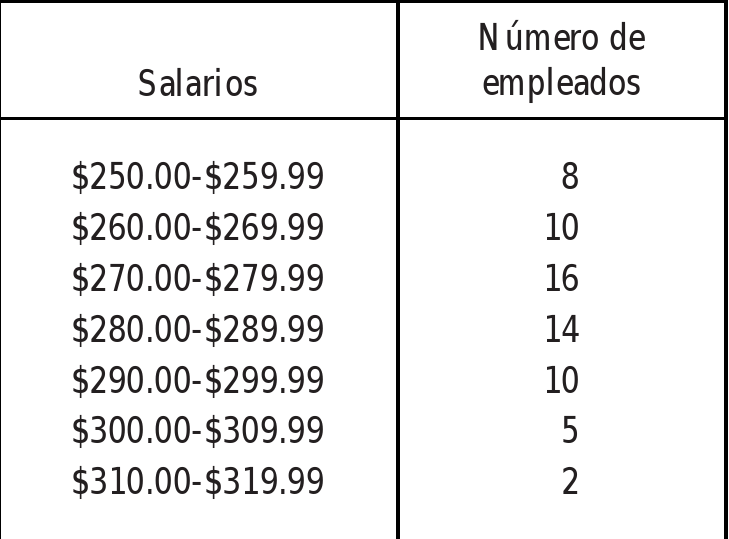
\includegraphics[height=5cm]{./images/tab0205.png}
		% tab0205.png: 0x0 pixel, 300dpi, 0.00x0.00 cm, bb=
		\label{tab:0205}
	\end{figure}
	
\end{problema}

